
\chapter{Week 2 -- BMS Temperature Stability}
\section{Abstract}
This report presents the results of measurements required by the assignment\footnote{accesiable via \url{https://moodle.fel.cvut.cz/pluginfile.php/474390/mod_resource/content/0/CV02_BMS.pdf}}. The laboratory task focuses on the temperature stability of the voltage threshold of three distinct cell balancing circuits. Their U-I characteristics were measured at various temperatures to assess the variability of voltage thresholds in real applications.


\section{Experimental setup}

\IEEEPARstart{T}{he} set of three cell balancing circuits -- devices under test -- with cell connection pads exposed as marked wires was enclosed into a box with a heating element and a thermometer. The voltage-current characteristics of individual devices were measured at several temperatures. Each measurement was performed manually using a programmable power supply used in the constant current operating mode. For each specified value of the discharging current, the corresponding voltage reading was recorded. This method suffered from inaccuracy by neglecting some factors, such as the wire resistance. Furthermore, the power supply only provides voltage readings with a resolution of 1 mV, which was insufficient to obtain more detailed U-I characteristics in the proximity of threshold voltage. Therefore the U-I characteristic is assumed to be piecewise linear in two regions
\begin{equation}
    i(u) = \begin{cases}
    0 & \text{if }  u < u_{\rm{T}}, \\
    \frac{u - u_{\rm{T}}}{R} & \text{if }  u \ge u_{\rm{T}},
    \end{cases}
\end{equation}
where $u_{\rm{T}}$ is the threshold voltage.

\section{Experimental results and conclusions}




\begin{figure}[htbp]
    \centering
    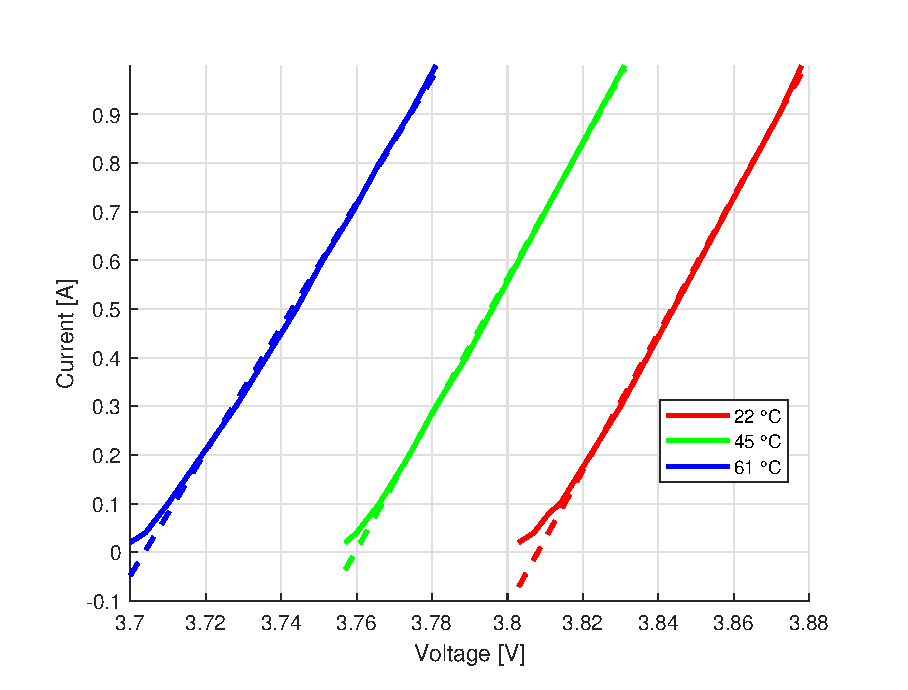
\includegraphics[width=0.5\linewidth]{figures/2/sample_A.eps}
    \caption{U-I characteristic of sample A}
    \label{fig:2-sample-A}
\end{figure}

Measured voltage-current characteristics of sample A for various temperatures are shown in Fig. \ref{fig:2-sample-A} together with their corresponding linear approximations. The threshold voltage is calculated as the x-intercept of the linear approximation. It is clear that the threshold voltage significantly varies with temperature approximately according to
\begin{equation}
    u_{\rm T} (\theta) \approx -0.0026~\theta + 3.8695 \text{ V},
\end{equation}
where $\theta$ is the temperature in °C.

Results for sample B are shown in Fig. \ref{fig:2-sample-B}, hinting that this sample is far more stable than sample B. The approximate temperature dependence of the threshold voltage is
\begin{equation}
    u_{\rm T} (\theta) \approx -0.0002~\theta + 3.9481 \text{ V},
\end{equation}
so more than an order of magnitude more stable.

\begin{figure}[htbp]
    \centering
    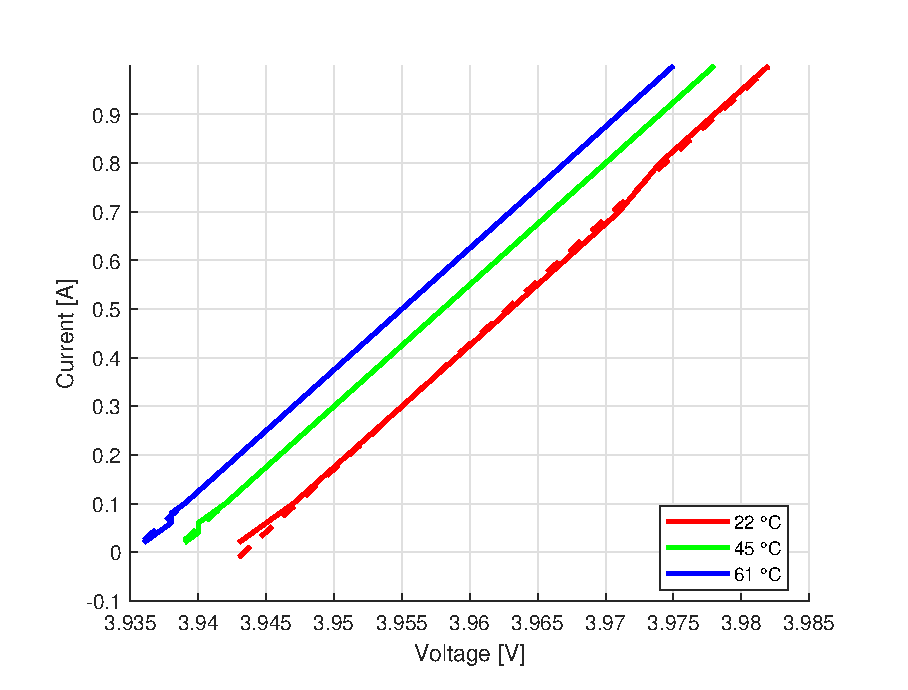
\includegraphics[width=0.5\linewidth]{figures/2/sample_B.eps}
    \caption{U-I characteristic of sample B}
    \label{fig:2-sample-B}
\end{figure}

No characteristics were measured for the sample C, as that BMS employed digital control via an integrated circuit, making it impossible to measure any static characteristic, as the discharge resistor was switched at irregular intervals according to the BMs internal logic.

